\PassOptionsToPackage{table}{xcolor}
\documentclass[aspectratio=169,12pt]{beamer}
\usepackage[T1]{fontenc}
\usepackage{lmodern}
\usepackage{tikz}
\usetikzlibrary{arrows,positioning,fit,backgrounds,decorations.pathreplacing}
\usepackage{xcolor}
\usepackage{array}
\usepackage{mdframed}
\usepackage{listings}
\lstset{
  basicstyle=\ttfamily\footnotesize,
  keywordstyle=\color{Navy}\bfseries,
  commentstyle=\color{MidGray}\itshape,
  backgroundcolor=\color{NavyDk!6},
  frame=single, framerule=0pt,
  xleftmargin=6pt, xrightmargin=6pt,
  aboveskip=2pt, belowskip=1pt,
  breaklines=true, breakatwhitespace=true,
  language=C
}

\definecolor{NavyDk}{HTML}{0D1B2A}
\definecolor{Navy}{HTML}{1B3A6B}
\definecolor{Teal}{HTML}{0A7C7B}
\definecolor{Orange}{HTML}{E8921A}
\definecolor{SlideGray}{HTML}{EEF3F8}
\definecolor{MidGray}{HTML}{5A6070}
\definecolor{LtGray}{HTML}{C0C8D8}
\definecolor{BoxGray}{HTML}{5A6880}
\definecolor{GreenHi}{HTML}{2A7A3A}

\usetheme{default}
\setbeamersize{text margin left=0.8cm,text margin right=0.8cm}
\setbeamertemplate{navigation symbols}{}
\setbeamercolor{background canvas}{bg=SlideGray}
\setbeamercolor{frametitle}{fg=Navy,bg=SlideGray}
\setbeamerfont{frametitle}{size=\large,series=\bfseries}
\setbeamertemplate{frametitle}{%
  \vspace{0.08cm}%
  {\usebeamerfont{frametitle}\usebeamercolor[fg]{frametitle}\insertframetitle}\\[-4pt]%
  {\color{Orange}\rule{\textwidth}{2.5pt}}%
}
\setbeamertemplate{footline}{%
  \vspace{2pt}%
  \hspace{0.6cm}{\color{MidGray}\fontsize{7.5}{9}\selectfont
    Hardware / Software Codesign \enspace|\enspace 2025/26 \enspace|\enspace IST}%
  \hfill%
  {\color{MidGray}\fontsize{7.5}{9}\selectfont\insertframenumber}%
  \hspace{0.5cm}\vspace{1pt}%
}

\begin{document}

%% SLIDE 1
{
\setbeamercolor{background canvas}{bg=NavyDk}
\setbeamertemplate{footline}{%
  \vspace{2pt}%
  \hspace{0.6cm}{\color{LtGray}\fontsize{7.5}{9}\selectfont
    Hardware / Software Codesign \enspace|\enspace 2025/26 \enspace|\enspace IST}%
  \hfill%
  {\color{LtGray}\fontsize{7.5}{9}\selectfont\insertframenumber}%
  \hspace{0.5cm}\vspace{1pt}%
}
\begin{frame}[plain]
  \vspace{0.2cm}
  \begin{center}
    {\color{white}\fontsize{32}{38}\selectfont\textbf{Fixed-Point Arithmetic}}\\[0.15cm]
    {\color{Orange}\fontsize{22}{26}\selectfont\textbf{\& Quantisation}}\\[0.4cm]
    {\color{LtGray}\fontsize{11}{14}\selectfont
      L7 \enspace$\cdot$\enspace Week 5 \enspace$\cdot$\enspace
      Hardware / Software Codesign 2025/26}\\[0.1cm]
    {\color{LtGray}\fontsize{10}{12}\selectfont
      Jos\'{e} T.\ de Sousa \enspace$\cdot$\enspace IST}
  \end{center}
  \vspace{0.15cm}
  \begin{center}
  
\begin{tikzpicture}[
    box/.style={rounded corners=3pt, minimum width=2.8cm, minimum height=1.1cm,
                align=center, font=\small\bfseries},
    node distance=0.35cm
  ]
    \node[box, fill=BoxGray,  text=white] (a) {Range\\{\normalfont\fontsize{8}{10}\selectfont integer bits $I$}};
    \node[box, fill=Navy,     text=white, right=of a] (b) {Precision\\{\normalfont\fontsize{8}{10}\selectfont fractional bits $W{-}I$}};
    \node[box, fill=Orange,   text=white, right=of b] (c) {Quantisation\\{\normalfont\fontsize{8}{10}\selectfont SNR / RMSE}};
    \node[box, fill=Teal,     text=white, right=of c] (d) {\texttt{ap\_fixed}\\{\normalfont\fontsize{8}{10}\selectfont methodology}};
  \end{tikzpicture}
  \end{center}
  \vspace{0.1cm}
  \begin{center}
    {\color{LtGray}\itshape\fontsize{10}{12}\selectfont
      How many bits are enough --- and how do you know?}
  \end{center}
\end{frame}
}

%% SLIDE 2
\begin{frame}{Where We Are}
\vspace{0.05cm}
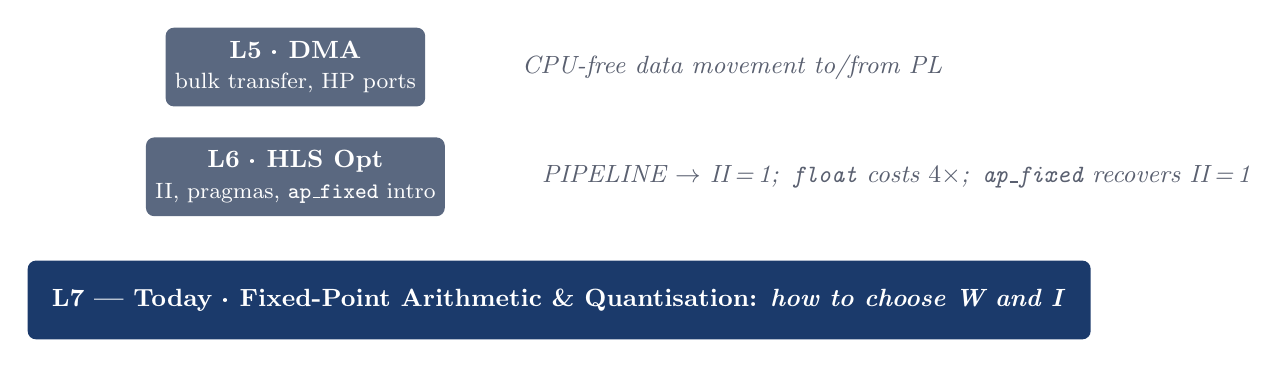
\begin{tikzpicture}[
  lbl/.style={rounded corners=3pt, minimum width=2.8cm, minimum height=1.0cm,
              align=center, font=\small\bfseries, text=white},
  note/.style={align=left, font=\small\itshape, text=MidGray},
  node distance=0.38cm
]
  \node[lbl, fill=BoxGray] (l5)
    {\textbf{L5} \textperiodcentered\ DMA\\
     {\normalfont\fontsize{8}{10}\selectfont bulk transfer, HP ports}};
  \node[lbl, fill=BoxGray, below=of l5] (l6)
    {\textbf{L6} \textperiodcentered\ HLS Opt\\
     {\normalfont\fontsize{8}{10}\selectfont II, pragmas, \texttt{ap\_fixed} intro}};
  \node[note, right=1.1cm of l5] {CPU-free data movement to/from PL};
  \node[note, right=1.1cm of l6]
    {PIPELINE $\to$ II\,=\,1;\enspace \texttt{float} costs $4\times$;\enspace
     \texttt{ap\_fixed} recovers II\,=\,1};
  \node[lbl, fill=Navy, minimum width=13.5cm, minimum height=1.0cm,
        below=0.55cm of l6, xshift=3.35cm]
    {\textbf{L7 --- Today} \textperiodcentered\
     Fixed-Point Arithmetic \& Quantisation: \emph{how to choose W and I}};
\end{tikzpicture}
\vspace{0.1cm}
{\color{Teal}\itshape\small
  L6 gave us the \texttt{ap\_fixed} syntax and showed it recovers II\,=\,1.
  Today we answer the harder question:
  \textbf{how do you choose W and I for your algorithm?}}
\end{frame}

%% SLIDE 3
\begin{frame}[t]{Today's Question}
\vspace{0.07cm}
\begin{center}
  \colorbox{NavyDk}{\parbox{0.82\textwidth}{%
    \vspace{4pt}
    \centering
    {\color{white}\fontsize{18}{22}\selectfont\bfseries
      ``How many bits are enough?''}\\[1pt]
    {\color{LtGray}\fontsize{10}{13}\selectfont
      Too few $\;\Rightarrow\;$ overflow or unacceptable rounding error.\quad
      Too many $\;\Rightarrow\;$ wasted LUTs and DSPs.}
    \vspace{4pt}
  }}
\end{center}
\vspace{0.11cm}
\begin{columns}[T,totalwidth=\textwidth]
  \column{0.49\textwidth}
  \colorbox{Orange!10}{\parbox{\dimexpr\linewidth-2\fboxsep\relax}{%
    \vspace{2pt}
    {\color{Orange}\bfseries What we already know (L6)}\\[1pt]
    {\footnotesize\color{Navy}
    \begin{itemize}\setlength{\itemsep}{1pt}
      \item \texttt{ap\_fixed<W,I>} syntax and types
      \item Fixed-point gives II\,=\,1 vs.\ float II\,=\,4
      \item Area \& accuracy trade-off exists
    \end{itemize}}
    \vspace{1pt}
  }}
  \column{0.02\textwidth}
  \column{0.49\textwidth}
  \colorbox{Teal!10}{\parbox{\dimexpr\linewidth-2\fboxsep\relax}{%
    \vspace{2pt}
    {\color{Teal}\bfseries What L7 adds}\\[1pt]
    {\footnotesize\color{Navy}
    \begin{itemize}\setlength{\itemsep}{1pt}
      \item Quantisation error: how to measure it
      \item Word-length optimisation methodology
      \item Fixed-point C++ simulation \& testbench
      \item Case study: FIR filter in \texttt{ap\_fixed}
    \end{itemize}}
    \vspace{1pt}
  }}
\end{columns}
\end{frame}

%% SLIDE 4
\begin{frame}{Lecture Roadmap}
\vspace{0.07cm}
\resizebox{\textwidth}{!}{%
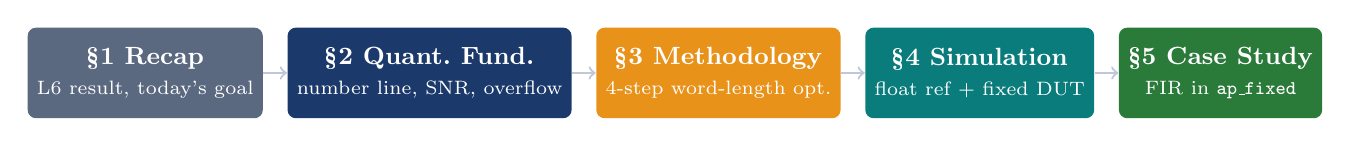
\begin{tikzpicture}[
  sbox/.style={rounded corners=3pt, minimum width=2.5cm, minimum height=1.15cm,
               align=center, font=\small\bfseries, text=white},
  node distance=0.3cm
]
  \node[sbox, fill=BoxGray]             (s1)
    {\S1 Recap\\{\normalfont\fontsize{7.5}{9}\selectfont L6 result, today's goal}};
  \node[sbox, fill=Navy,   right=of s1] (s2)
    {\S2 Quant.\ Fund.\\{\normalfont\fontsize{7.5}{9}\selectfont number line, SNR, overflow}};
  \node[sbox, fill=Orange, right=of s2] (s3)
    {\S3 Methodology\\{\normalfont\fontsize{7.5}{9}\selectfont 4-step word-length opt.}};
  \node[sbox, fill=Teal,   right=of s3] (s4)
    {\S4 Simulation\\{\normalfont\fontsize{7.5}{9}\selectfont float ref + fixed DUT}};
  \node[sbox, fill=GreenHi,right=of s4] (s5)
    {\S5 Case Study\\{\normalfont\fontsize{7.5}{9}\selectfont FIR in \texttt{ap\_fixed}}};
  \draw[->, thick, color=LtGray] (s1.east) -- (s2.west);
  \draw[->, thick, color=LtGray] (s2.east) -- (s3.west);
  \draw[->, thick, color=LtGray] (s3.east) -- (s4.west);
  \draw[->, thick, color=LtGray] (s4.east) -- (s5.west);
\end{tikzpicture}}
\vspace{0.15cm}
\begin{center}
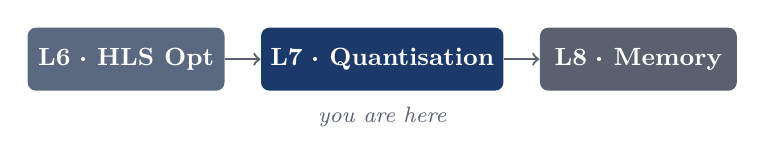
\begin{tikzpicture}[
  lbl/.style={rounded corners=3pt, minimum width=2.5cm, minimum height=0.8cm,
              align=center, font=\small\bfseries, text=white},
  node distance=0.45cm
]
  \node[lbl, fill=BoxGray]            (l6) {L6 \textperiodcentered\ HLS Opt};
  \node[lbl, fill=Navy,  right=of l6] (l7) {L7 \textperiodcentered\ Quantisation};
  \node[lbl, fill=MidGray,right=of l7](l8) {L8 \textperiodcentered\ Memory};
  \draw[->, thick, color=MidGray] (l6.east) -- (l7.west);
  \draw[->, thick, color=MidGray] (l7.east) -- (l8.west);
  \node[font=\footnotesize\itshape, text=MidGray, below=0.08cm of l7]
    {you are here};
\end{tikzpicture}
\end{center}
\end{frame}

%% SLIDE 5
\begin{frame}[t]{The Fixed-Point Number Line}
\vspace{0.04cm}
\begin{columns}[T,totalwidth=\textwidth]
  \column{0.50\textwidth}
  \vspace{1.02cm}
  \begin{tikzpicture}[scale=0.70]
    \draw[<->, thick, Navy] (-0.3,0) -- (8.8,0);
    \foreach \x in {0,0.5,...,7.5}
      \draw[thick, Navy] (\x+0.25, 0.1) -- (\x+0.25, -0.1);
    \node[font=\tiny\color{NavyDk}, below=0.1cm] at (0.25,0)  {$-2$};
    \node[font=\tiny\color{NavyDk}, below=0.1cm] at (2.25,0)  {$-1$};
    \node[font=\tiny\color{NavyDk}, below=0.1cm] at (4.25,0)  {$0$};
    \node[font=\tiny\color{NavyDk}, below=0.1cm] at (6.25,0)  {$1$};
    \node[font=\tiny\color{NavyDk}, below=0.1cm] at (7.75,0)  {$1\tfrac{3}{4}$};
    \draw[<->, thick, Orange]
      (4.25, 0.4) -- (4.75, 0.4)
      node[midway, above, font=\scriptsize\color{Orange}]
        {LSB $= \tfrac{1}{4}$};
    \draw[decorate,
          decoration={brace, amplitude=4pt, raise=0.35cm},
          thick, Teal]
      (0.25,1.43) -- (7.75,1.43)
      node[midway, above=0.45cm, font=\scriptsize\color{Teal}]
        {Range $= 2^{I} = 4$};
    \node[rounded corners=3pt, fill=Navy!12, font=\scriptsize\color{Navy},
          inner sep=2pt] at (4.0,-0.70)
      {\texttt{ap\_fixed<4,2>}: $W{=}4$ total bits,\; $I{=}2$ integer bits};
  \end{tikzpicture}
  \column{0.50\textwidth}
  \vspace{0.02cm}
  {\color{Navy}\bfseries\small Two parameters control everything:}
  \vspace{1pt}
  {\footnotesize\begin{itemize}\setlength{\itemsep}{1pt}
    \item[\color{Orange}$\blacktriangleright$]
      \textbf{$I$ (integer bits):} range
      $\bigl[-2^{I-1},\; 2^{I-1}{-}\text{LSB}\bigr]$
    \item[\color{Teal}$\blacktriangleright$]
      \textbf{$W{-}I$ (frac.\ bits):}
      $\text{LSB} = 2^{I-W}$
    \item[\color{Navy}$\blacktriangleright$]
      \textbf{Max error} $\leq \tfrac{\text{LSB}}{2}$ (with rounding)
    \item[\color{BoxGray}$\blacktriangleright$]
      Each extra frac.\ bit \textbf{halves} error
      (+1 bit of hardware)
  \end{itemize}}
  \vspace{2pt}
  \colorbox{Orange!12}{\parbox{\dimexpr\linewidth-2\fboxsep\relax}{%
    \vspace{1pt}
    {\footnotesize\color{NavyDk}
      \textbf{Goal:} smallest $W$ meeting your error target.}
    \vspace{1pt}
  }}
\end{columns}
\end{frame}

%% SLIDE 6
\begin{frame}[t,fragile]{Truncation vs.\ Rounding}
\vspace{0.05cm}
\begin{columns}[T,totalwidth=\textwidth]
  \column{0.49\textwidth}
  \colorbox{Orange!10}{\parbox{\dimexpr\linewidth-2\fboxsep\relax}{%
    \vspace{2pt}
    {\color{Orange}\bfseries AP\_TRN --- Truncation (default)}\\[1pt]
    {\footnotesize\color{Navy} Drop the extra bits --- equivalent to floor.}\\[1pt]
    {\small
    \begin{itemize}\setlength{\itemsep}{1pt}
      \item Error range: $[-\text{LSB},\; 0)$
      \item \textbf{Biased} --- average error $= -\tfrac{\text{LSB}}{2}$
      \item Free in hardware: no extra logic
    \end{itemize}}
    \vspace{1pt}
  }}
  \column{0.02\textwidth}
  \column{0.49\textwidth}
  \colorbox{Teal!10}{\parbox{\dimexpr\linewidth-2\fboxsep\relax}{%
    \vspace{2pt}
    {\color{Teal}\bfseries AP\_RND --- Round to Nearest}\\[1pt]
    {\footnotesize\color{Navy} Add $\tfrac{\text{LSB}}{2}$ before truncating.}\\[1pt]
    {\small
    \begin{itemize}\setlength{\itemsep}{1pt}
      \item Error range: $\bigl[-\tfrac{\text{LSB}}{2},\; +\tfrac{\text{LSB}}{2}\bigr)$
      \item \textbf{Unbiased} --- zero mean error
      \item Costs one adder in hardware
    \end{itemize}}
    \vspace{1pt}
  }}
\end{columns}
\vspace{0.1cm}
\begin{lstlisting}
ap_fixed<8,4, AP_TRN> a = 3.17f;  // Stored as 3.125
ap_fixed<8,4, AP_RND> b = 3.17f;  // Stored as 3.1875
\end{lstlisting}
\vspace{0.07cm}
{\small\color{MidGray}\itshape
  Rule of thumb: use \texttt{AP\_RND} unless area is critical ---
  the extra adder is negligible compared to the accuracy gain.}
\end{frame}

%% SLIDE 7
\begin{frame}[t,fragile]{Overflow and Saturation}
\vspace{0.05cm}
\begin{columns}[T,totalwidth=\textwidth]
  \column{0.49\textwidth}
  \colorbox{Orange!10}{\parbox{\dimexpr\linewidth-2\fboxsep\relax}{%
    \vspace{2pt}
    {\color{Orange}\bfseries AP\_WRAP --- Wrap-around}\\[1pt]
    {\footnotesize\color{Navy}
      Modular arithmetic: value wraps from MAX to MIN.}\\[1pt]
    {\footnotesize
    \begin{itemize}\setlength{\itemsep}{1pt}
      \item Free: discard the carry-out bit
      \item Catastrophic if overflow is unexpected
      \item Use only when overflow is \emph{provably impossible}
    \end{itemize}}
    \vspace{1pt}
  }}
  \column{0.02\textwidth}
  \column{0.49\textwidth}
  \colorbox{Teal!10}{\parbox{\dimexpr\linewidth-2\fboxsep\relax}{%
    \vspace{2pt}
    {\color{Teal}\bfseries AP\_SAT --- Saturate}\\[1pt]
    {\footnotesize\color{Navy}
      Clamp to $[\text{MIN},\; \text{MAX}]$ on overflow.}\\[1pt]
    {\footnotesize
    \begin{itemize}\setlength{\itemsep}{1pt}
      \item Costs a comparator and mux
      \item Graceful degradation --- no sign flip
      \item Required for audio, image, control loops
    \end{itemize}}
    \vspace{1pt}
  }}
\end{columns}
\vspace{0.02cm}
\begin{lstlisting}
ap_fixed<8,4, AP_RND, AP_WRAP> w;  w = 7.9f;  // wraps to -8
ap_fixed<8,4, AP_RND, AP_SAT>  s;  s = 7.9f;  // clamps to 7.875
\end{lstlisting}
\vspace{0.02cm}
{\footnotesize\color{MidGray}\itshape
  Default is \texttt{AP\_WRAP}.
  Always use \texttt{AP\_SAT} for outputs that feed audio codecs,
  pixel pipelines, or PID controllers.}
\end{frame}

%% SLIDE 8
\begin{frame}[t,fragile]{Full \texttt{ap\_fixed} Template}
\vspace{0.01cm}
\begin{center}
\colorbox{NavyDk}{\parbox{0.9\textwidth}{%
  \vspace{2pt}\centering
  {\color{Orange}\ttfamily\normalsize ap\_fixed\,<\,W,\;I,\;Q,\;O\,>}\\
  {\color{LtGray}\footnotesize
    total bits \hspace{1.2cm} integer bits
    \hspace{0.9cm} quantise mode
    \hspace{0.6cm} overflow mode}
  \vspace{2pt}
}}
\end{center}
\vspace{0.02cm}
{\setlength{\extrarowheight}{0pt}
{\small\begin{tabular}{>{\ttfamily\bfseries}p{1.4cm}p{3.2cm}p{7.5cm}}
\rowcolor{Navy!15}
\textbf{Param} & \textbf{Common values} & \textbf{Meaning}\\
W & 8, 12, 16, 24 & Total word width in bits\\
I & 1, 2, 4, \ldots & Integer bits (including sign); sets range\\
Q & AP\_TRN, AP\_RND, AP\_RND\_CONV & What to do when dropping LSBs (conv.\ = banker's rounding)\\
O & AP\_WRAP, AP\_SAT & What to do when value exceeds range\\
\end{tabular}}}
\vspace{0.02cm}
\begin{lstlisting}[basicstyle=\ttfamily\scriptsize,aboveskip=1pt,belowskip=0pt]
// Typical project typedefs
typedef ap_fixed<16, 2, AP_RND, AP_SAT>  pixel_t;  // image [-2,2)
typedef ap_fixed<16, 1, AP_RND, AP_SAT>  audio_t;  // audio [-1,1)
typedef ap_fixed<24, 5, AP_RND, AP_SAT>  accum_t;  // accumulator
\end{lstlisting}
\vspace{0.01cm}
{\scriptsize\color{MidGray}\itshape
  Signed (\texttt{ap\_fixed}) is the default.
  Use \texttt{ap\_ufixed} for quantities that are always non-negative.}
\end{frame}

%% SLIDE 9
\begin{frame}[t]{Quantisation Noise and SNR}
\vspace{0.04cm}
\setlength{\abovedisplayskip}{2pt}\setlength{\belowdisplayskip}{2pt}%
\begin{columns}[T,totalwidth=\textwidth]
  \column{0.52\textwidth}
  \vspace{0.02cm}
  {\color{Navy}\bfseries Signal-to-Noise Ratio (SNR)}
  \[
    \text{SNR} = 10\log_{10}\!\left(\frac{\sigma^2_{\text{signal}}}{\sigma^2_{\text{noise}}}\right) \;\text{[dB]}
  \]
  For \textbf{uniform quantisation with rounding}:
  \[
    \sigma^2_{\text{noise}} = \frac{\text{LSB}^2}{12}
    \quad\Rightarrow\quad
    \sigma^2_{\text{noise}} = \frac{2^{2(I-W)}}{12}
  \]
  For a full-scale sinusoid ($\sigma^2_s = A^2/2$):
  \[
    \text{SNR} \approx 6.02\,(W - I) + 1.76\;\text{dB}
  \]
  {\small\color{Orange}\bfseries Each extra fractional bit adds $\approx$6\,dB.}
  \column{0.48\textwidth}
  \vspace{0.02cm}
  {\color{Navy}\bfseries Typical targets:}
  \vspace{1pt}
  {\setlength{\extrarowheight}{0pt}
  \begin{tabular}{lrl}
  \rowcolor{Navy!15}
  \textbf{Application} & \textbf{Target} & \textbf{Min bits}\\
  Studio audio  & $\sim$144\,dB & 24\\
  CD audio      & $\sim$96\,dB  & 16\\
  Image proc.\  & 40\,dB        & 7\\
  Control loop  & 30\,dB        & 5\\
  \end{tabular}}
  \vspace{0.02cm}
  \colorbox{Teal!12}{\parbox{\dimexpr\linewidth-2\fboxsep\relax}{%
    \vspace{1pt}
    {\footnotesize\color{NavyDk}
      \textbf{In practice:} always \emph{measure} SNR
      in a C testbench with real data.
      The formula assumes uniform signal
      distribution --- your data may differ.}
    \vspace{1pt}
  }}
\end{columns}
\end{frame}

%% SLIDE 10
\begin{frame}[t,fragile]{Common \texttt{ap\_fixed} Pitfalls}
\vspace{0.04cm}
\begin{columns}[T,totalwidth=\textwidth]
  \column{0.49\textwidth}
  {\color{Orange}\bfseries Pitfall 1 --- Accumulator overflow}\\[1pt]
  {\small After $N$ multiply-accumulates, the result can be $N\times$ larger than one term.
  Add $\lceil\log_2 N\rceil$ extra integer bits:}
  \vspace{2pt}
\begin{lstlisting}
// 16-tap FIR, data in [-1,1)
// product in [-1,1): I=1
// sum of 16: max=16, need I=5
typedef ap_fixed<16,1> data_t;
typedef ap_fixed<20,5> acc_t; // +4 bits
\end{lstlisting}
  \column{0.02\textwidth}
  \column{0.49\textwidth}
  {\color{Teal}\bfseries Pitfall 2 --- Silent narrowing}\\[1pt]
  {\small Assigning a wide type to a narrow one silently drops bits.
  HLS will not error --- check the synthesis log:}
  \vspace{2pt}
\begin{lstlisting}
acc_t  acc = compute();   // wide
data_t out = acc;  // SILENT truncation
// Fix: explicit cast or resize
data_t out = (data_t)acc;
\end{lstlisting}
\end{columns}
\vspace{0.1cm}
\colorbox{Orange!10}{\parbox{\textwidth}{%
  \vspace{1pt}
  {\small\color{NavyDk}
    \textbf{Rule:} after writing your HLS function, search the Vitis~HLS log for
    \texttt{WARNING: [XFORM]} width-change messages before trusting the output.}
  \vspace{1pt}
}}
\end{frame}

%% SLIDE 11
\begin{frame}{Section 3 --- Word-Length Optimisation Methodology}
\vspace{0.07cm}
{\color{MidGray}\small\itshape
  We know what \texttt{ap\_fixed} parameters mean.
  Now: a systematic way to \emph{choose} them.}
\vspace{0.13cm}
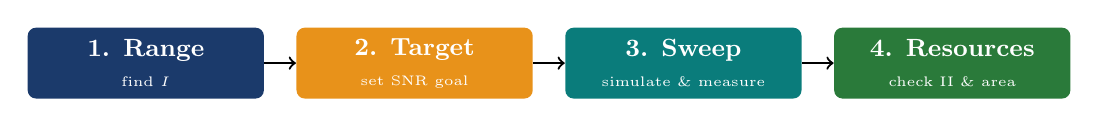
\begin{tikzpicture}[
  stbox/.style={rounded corners=3pt, minimum width=3.0cm, minimum height=0.9cm,
                align=center, font=\small\bfseries, text=white},
  node distance=0.4cm
]
  \node[stbox, fill=Navy]             (t1) {1. Range\\{\normalfont\tiny find $I$}};
  \node[stbox, fill=Orange, right=of t1] (t2) {2. Target\\{\normalfont\tiny set SNR goal}};
  \node[stbox, fill=Teal,   right=of t2] (t3) {3. Sweep\\{\normalfont\tiny simulate \& measure}};
  \node[stbox, fill=GreenHi,right=of t3] (t4) {4. Resources\\{\normalfont\tiny check II \& area}};
  \draw[->, thick] (t1.east) -- (t2.west);
  \draw[->, thick] (t2.east) -- (t3.west);
  \draw[->, thick] (t3.east) -- (t4.west);
\end{tikzpicture}
\vspace{0.13cm}
\begin{itemize}\setlength{\itemsep}{2pt}
  \item[\color{Navy}$\blacktriangleright$]
    \textbf{Step 1:} profile your float reference to find the dynamic range
  \item[\color{Orange}$\blacktriangleright$]
    \textbf{Step 2:} define the accuracy requirement for your application
  \item[\color{Teal}$\blacktriangleright$]
    \textbf{Step 3:} sweep $W$ in C simulation, measure SNR or RMSE
  \item[\color{GreenHi}$\blacktriangleright$]
    \textbf{Step 4:} synthesise the chosen $W$; verify II\,=\,1 and area budget
\end{itemize}
\end{frame}

%% SLIDE 12
\begin{frame}[t,fragile]{Step 1 --- Sizing the Integer Part ($I$ bits)}
\vspace{0.04cm}
\begin{columns}[T,totalwidth=\textwidth]
  \column{0.52\textwidth}
  {\color{Navy}\bfseries Find the dynamic range first:}
  \vspace{2pt}
\begin{lstlisting}
// Run float reference; record extremes
float max_abs = 0;
for (int n = 0; n < N; n++) {
  float v = compute_float(x, n);
  if (fabsf(v) > max_abs)
    max_abs = fabsf(v);
}
// Size I to cover max_abs with margin
int I = (int)ceilf(log2f(max_abs)) + 2;
\end{lstlisting}
  \column{0.48\textwidth}
  \vspace{0.04cm}
  {\color{Navy}\bfseries Formula:}
  \[
    I = \lceil \log_2 V_{\max} \rceil + 1 \;(\text{sign}) + 1\;(\text{guard})
  \]
  \vspace{0.07cm}
  {\color{Navy}\bfseries Examples:}
  \vspace{1pt}
  {\setlength{\extrarowheight}{1pt}
  \begin{tabular}{lrl}
  \rowcolor{Navy!15}
  \textbf{Signal} & $V_{\max}$ & $I$ \\
  Audio $[-1,1)$      & 1    & 2 \\
  GEMM row ($n{=}64$) & 64   & 8 \\
  FIR output ($N{=}16$)& 16  & 6 \\
  \end{tabular}}
  \vspace{0.08cm}
  \colorbox{Orange!12}{\parbox{\dimexpr\linewidth-2\fboxsep\relax}{%
    \vspace{1pt}
    {\small\color{NavyDk}
      Always add \textbf{1--2 guard bits} above the measured
      maximum. Corner-case inputs may exceed your training set.}
    \vspace{1pt}
  }}
\end{columns}
\end{frame}

%% SLIDE 13
\begin{frame}[t,fragile]{Word-Length Methodology: Vary \texttt{FIN} in C-sim}
\vspace{0.04cm}
\begin{columns}[T,totalwidth=\textwidth]
  \column{0.46\textwidth}
  {\color{Navy}\bfseries Signal representations derived from \texttt{IIN}:}
  \vspace{2pt}
  {\scriptsize\setlength{\extrarowheight}{1pt}
  \begin{tabular}{lp{3.2cm}}
  \rowcolor{Navy!15}
  \textbf{Signal} & \textbf{Format}\\
  Input / coeff  & \texttt{ap\_fixed<WIN,IIN>}\\
  Product        & \texttt{ap\_fixed<2*WIN,2*IIN>}\\
  Accumulator    & \texttt{ap\_fixed<2*WIN+G,2*IIN+G>}\\
  \end{tabular}}
  \vspace{0.07cm}
  {\small\color{NavyDk}
  Change \texttt{\#define FIN} and rerun \texttt{csim\_design}.\\
  Measure max error vs.\ \texttt{double} baseline.\\
  Choose smallest \texttt{FIN} meeting error target.}
  \column{0.54\textwidth}
  \vspace{0.04cm}
\begin{lstlisting}
#define IIN  1   // range [-1,1)
#define FIN  12  // vary this
#define WIN  (FIN+IIN)
#define G    4   // log2(16 taps)
typedef ap_fixed<WIN,   IIN>   data_t;
typedef ap_fixed<2*WIN, 2*IIN> mul_t;
typedef ap_fixed<2*WIN+G,2*IIN+G> acc_t;
// testbench: compare with float ref
double err = fabs(hw_y - ref_y);
\end{lstlisting}
\end{columns}
\end{frame}

%% SLIDE 14 -- Arithmetic format rules
\begin{frame}[t]{\texttt{ap\_fixed} Arithmetic --- Format Propagation Rules}
\vspace{0.06cm}
{\small\color{MidGray}\itshape
  When two \texttt{ap\_fixed} values are combined, the result format follows
  these rules. HLS applies them automatically.}
\vspace{0.1cm}
{\setlength{\extrarowheight}{3pt}
\begin{tabular}{p{2.8cm}p{3.4cm}p{3.2cm}p{2.8cm}}
\rowcolor{Navy}
\textbf{\color{white}Operation} &
\textbf{\color{white}Integer bits} &
\textbf{\color{white}Frac.\ bits} &
\textbf{\color{white}Example}\\
\textbf{Add/Sub} $R = A \pm B$ &
$I_R = \max(I_A, I_B)+1$ &
$F_R = \max(F_A, F_B)$ &
{\small\texttt{<7,3>+<5,2>} $\to$ \texttt{<8,4>}}\\
\rowcolor{Navy!8}
\textbf{Multiply} $M = A \times B$ &
$I_M = I_A + I_B$ &
$F_M = F_A + F_B$ &
{\small\texttt{<7,3>*<5,2>} $\to$ \texttt{<12,5>}}\\
\textbf{Divide} $D = A \,/\, B$ &
$I_D = I_A + F_B$ &
$F_D = F_A$ &
{\small\texttt{<7,3>/<5,2>} $\to$ \texttt{<9,3>}}\\
\end{tabular}}
\vspace{0.08cm}
{\small\color{MidGray} Note: division requires extending dividend $A$ before the operation.}
\vspace{0.06cm}
\colorbox{Orange!10}{\parbox{\textwidth}{%
  \vspace{1pt}
  {\small\color{NavyDk}
    \textbf{Key insight:} multiplication grows the word fast ---
    \texttt{ap\_fixed<12,1>}$\times$\texttt{ap\_fixed<12,1>} needs a \texttt{<24,2>} result.
    Always accumulate into a wider type.}
  \vspace{1pt}
}}
\end{frame}

%% SLIDE 15 -- Bit and Range Operators
\begin{frame}[t,fragile]{\texttt{ap\_fixed} Bit and Range Operators}
\vspace{0.02cm}
\begin{columns}[T,totalwidth=\textwidth]
  \column{0.49\textwidth}
  \colorbox{Navy!10}{\parbox{\dimexpr\linewidth-2\fboxsep\relax}{%
    \vspace{1pt}
    {\color{Navy}\bfseries Bit operator \texttt{[i]}}\\[1pt]
    {\small Selects one bit. LSB has index 0.
    Returns a reference --- can read or write.}
    \vspace{1pt}
  }}
  \vspace{2pt}
\begin{lstlisting}[basicstyle=\ttfamily\scriptsize]
ap_fixed<8,5> v = 1.375; // 0b00001.011
v[3];        // 1  (bit 3 is set)
v[4];        // 0  (bit 4 is clear)
v[2] = 1;    // v becomes 1.875
v[3] = 0;    // v becomes 0.875
\end{lstlisting}
  \column{0.02\textwidth}
  \column{0.49\textwidth}
  \colorbox{Teal!10}{\parbox{\dimexpr\linewidth-2\fboxsep\relax}{%
    \vspace{1pt}
    {\color{Teal}\bfseries Range operator \texttt{(Hi,Lo)}}\\[1pt]
    {\small Selects a group of bits. If \texttt{Lo > Hi},
    bits are returned in reverse order.}
    \vspace{1pt}
  }}
  \vspace{2pt}
\begin{lstlisting}[basicstyle=\ttfamily\scriptsize]
ap_ufixed<4,2> u = 1.75; // 0b01.11
ap_uint<4> r, rev;
r   = u.range(3,0); // 7  (0b0111)
rev = u.range(0,3); // 14 (0b1110)
// Assign a slice from another variable:
ap_fixed<4,2> s;
ap_fixed<8,0> x = 0xAE;
s(3,0) = x(5,2);    // s = -1.25
\end{lstlisting}
\end{columns}
\end{frame}

%% SLIDE 16 -- printf for ap_fixed
\begin{frame}[t,fragile]{\texttt{ap\_fixed} Console Output --- \texttt{to\_string()} and \texttt{c\_str()}}
\vspace{0.02cm}
{\small\color{MidGray}\itshape
  For C-simulation, HLS supports printing \texttt{ap\_fixed} values in binary,
  decimal, or hexadecimal --- including values wider than 64 bits.}
\vspace{0.04cm}
\begin{columns}[T,totalwidth=\textwidth]
  \column{0.52\textwidth}
\begin{lstlisting}[basicstyle=\ttfamily\scriptsize]
ap_fixed<40,8> val = 112.1;
printf("binary:  %s\n",
       val.to_string().c_str());
printf("decimal: %s\n",
       val.to_string(10).c_str());
printf("hexa:    %s\n",
       val.to_string(16).c_str());
\end{lstlisting}
  \vspace{1pt}
  {\scriptsize\color{MidGray}
  \texttt{binary:\enspace 0b01110000.000110011...}\\
  \texttt{decimal: 112.0999999998603...}\\
  \texttt{hexa:\enspace\enspace 0x70.19999999p0}}
  \column{0.48\textwidth}
\begin{lstlisting}[basicstyle=\ttfamily\scriptsize]
// Signed/unsigned control:
ap_fixed<8,4> v = -5.25;
printf("%s\n",
  v.to_string(2).c_str());
  // 0b11010.1100
printf("%s\n",
  v.to_string(10).c_str());
  // -5.25
printf("%s\n",
  v.to_string(16, true).c_str());
  // -0x5.4p0  (signed)
printf("%s\n",
  v.to_string(16, false).c_str());
  // 0x1a.cp0  (unsigned)
\end{lstlisting}
\end{columns}
\vspace{0.02cm}
\colorbox{Orange!10}{\parbox{\textwidth}{%
  \vspace{1pt}
  {\small\color{NavyDk}
    \textbf{Use \texttt{to\_string()} only in testbenches} ---
    not in synthesisable HLS code. These calls are simulation-only.}
  \vspace{1pt}
}}
\end{frame}

%% SLIDE 17
\begin{frame}[t]{Step 4 --- Synthesis Check}
\vspace{0.05cm}
{\small Once the C simulation gives a passing $W$, run HLS synthesis and verify three things:}
\vspace{0.07cm}
\begin{columns}[T,totalwidth=\textwidth]
  \column{0.32\textwidth}
  \colorbox{Navy!10}{\parbox{\dimexpr\linewidth-2\fboxsep\relax}{%
    \vspace{2pt}
    {\color{Navy}\bfseries II still = 1?}\\[1pt]
    {\small Wider types need more DSP slices.
    If the Zynq runs out of DSPs, HLS serialises
    multiplications and II rises.
    Fix: reduce $W$ by 2 and re-check.}
    \vspace{2pt}
  }}
  \column{0.01\textwidth}
  \column{0.32\textwidth}
  \colorbox{Orange!10}{\parbox{\dimexpr\linewidth-2\fboxsep\relax}{%
    \vspace{2pt}
    {\color{Orange}\bfseries Area within budget?}\\[1pt]
    {\small Check the utilisation report: LUT, FF, DSP, BRAM.
    A $2\times$ increase in $W$ roughly doubles DSP usage
    for multiply-heavy kernels.}
    \vspace{2pt}
  }}
  \column{0.01\textwidth}
  \column{0.32\textwidth}
  \colorbox{Teal!10}{\parbox{\dimexpr\linewidth-2\fboxsep\relax}{%
    \vspace{2pt}
    {\color{Teal}\bfseries Timing closed?}\\[1pt]
    {\small Wider adders have longer critical paths.
    Confirm the post-synthesis report shows
    $\geq$100\,MHz.
    If not, reduce $W$ or add a pipeline stage.}
    \vspace{2pt}
  }}
\end{columns}
\vspace{0.1cm}
\colorbox{NavyDk!8}{\parbox{\textwidth}{%
  \vspace{1pt}
  {\small\color{NavyDk}
    \textbf{The trade-off curve:} as $W$ grows, SNR improves (good) but area and
    possibly II worsen (bad). Your job is to find the \emph{knee} of that curve.}
  \vspace{1pt}
}}
\end{frame}

%% SLIDE 18
\begin{frame}[t]{Practical Heuristics}
\vspace{0.04cm}
\begin{itemize}\setlength{\itemsep}{4pt}
  \item[\color{Orange}$\blacktriangleright$]
    \textbf{Accumulator width} after $N$ additions:
    \[
      W_{\text{acc}} = W_{\text{data}} + \lceil \log_2 N \rceil
      \qquad
      I_{\text{acc}} = I_{\text{data}} + \lceil \log_2 N \rceil
    \]
    {\small Example: 16-tap FIR, data \texttt{ap\_fixed<12,2>}
      $\;\Rightarrow\;$ accumulator \texttt{ap\_fixed<16,6>}}
  \item[\color{Teal}$\blacktriangleright$]
    \textbf{Multiplier output width} $= W_A + W_B$ bits.
    Always store in a type at least that wide before truncating.
  \item[\color{Navy}$\blacktriangleright$]
    \textbf{Coefficients} can usually be 2--4 bits narrower than the data type
    without significant SNR loss (they are constant and bounded).
  \item[\color{GreenHi}$\blacktriangleright$]
    \textbf{Start wide, narrow down.}
    Begin with $W = 24$ to confirm algorithm correctness,
    then reduce until SNR just meets the target.
  \item[\color{BoxGray}$\blacktriangleright$]
    \textbf{Read the HLS warnings.}
    \texttt{WARNING: [XFORM] ap\_fixed} width-change messages flag every
    silent truncation in your design.
\end{itemize}
\end{frame}

%% SLIDE 19
\begin{frame}{Section 4 --- Fixed-Point C\texttt{++} Simulation}
\vspace{0.05cm}
{\color{MidGray}\small\itshape
  Step 3 of the methodology requires simulating your fixed-point design in C\texttt{++}.
  Here is the pattern that makes it reliable.}
\vspace{0.11cm}
\begin{columns}[T,totalwidth=\textwidth]
  \column{0.49\textwidth}
  \colorbox{Navy!10}{\parbox{\dimexpr\linewidth-2\fboxsep\relax}{%
    \vspace{2pt}
    {\color{Navy}\bfseries Float reference}\\[1pt]
    {\small The ground truth. Implemented in \texttt{float} or \texttt{double}.
    Known correct. You already have this from the SW phase.}
    \vspace{2pt}
  }}
  \column{0.02\textwidth}
  \column{0.49\textwidth}
  \colorbox{Teal!10}{\parbox{\dimexpr\linewidth-2\fboxsep\relax}{%
    \vspace{2pt}
    {\color{Teal}\bfseries ap\_fixed DUT}\\[1pt]
    {\small The design under test. Same algorithm, types replaced
    with \texttt{ap\_fixed<W,I,...>}. Run on the same inputs.
    Compare outputs to the reference.}
    \vspace{2pt}
  }}
\end{columns}
\vspace{0.11cm}
\begin{itemize}\setlength{\itemsep}{2pt}
  \item[\color{Orange}$\blacktriangleright$]
    Run both on the \textbf{same inputs}: synthetic vectors, real data, or edge cases
  \item[\color{Navy}$\blacktriangleright$]
    Compute \textbf{SNR or RMSE} from the difference
  \item[\color{Teal}$\blacktriangleright$]
    Iterate $W$ in a loop --- C simulation is fast, no synthesis needed
\end{itemize}
\end{frame}

%% SLIDE 20
\begin{frame}[fragile]{Testbench Code Pattern}
\begin{lstlisting}[basicstyle=\ttfamily\scriptsize,aboveskip=1pt,belowskip=0pt]
#include "ap_fixed.h"
#include <math.h>
#define N 256
typedef ap_fixed<16,2, AP_RND, AP_SAT> fx_t;
float compute_float(float x); // float reference
fx_t  compute_fixed(fx_t  x);// ap_fixed DUT
int main() {
    float x_f[N];  fx_t x_fx[N];
    double err_sq = 0, sig_sq = 0;
    for (int n = 0; n < N; n++) {
        float ref = compute_float(x_f[n]);
        float dut = (float)compute_fixed(x_fx[n]);
        err_sq += (ref-dut)*(ref-dut);
        sig_sq += ref*ref;
    }
    float snr = 10.0f*log10f((float)(sig_sq/err_sq));
    printf("SNR = %.1f dB\n", snr);
    return (snr >= 60.0f) ? 0 : 1;
}
\end{lstlisting}
\end{frame}

%% SLIDE 21 -- Scale-and-Round sweep (inserted)
\begin{frame}[fragile]{Scale-and-Round: Sweeping $W$ Without Recompilation}
\vspace{0.02cm}
Quantise in pure C by multiplying by $S = 2^N$, rounding, then dividing back:
\begin{lstlisting}[basicstyle=\ttfamily\scriptsize,aboveskip=4pt,belowskip=4pt]
float quantize(float x, float S) {
    return roundf(x * S) / S;
}
\end{lstlisting}
Sweep all scale factors in one run --- no recompilation needed:
\begin{lstlisting}[basicstyle=\ttfamily\scriptsize,aboveskip=4pt,belowskip=4pt]
for (int N = 4; N <= 20; N++) {
    float S = powf(2.0f, (float)N);
    double err_sq = 0, sig_sq = 0;
    for (int i = 0; i < LEN; i++) {
        float q = quantize(ref[i], S);
        err_sq += (ref[i]-q)*(ref[i]-q);
        sig_sq += ref[i]*ref[i];
    }
    float snr = 10.0f*log10f((float)(sig_sq/err_sq));
    printf("N=%2d  SNR=%5.1f dB\n", N, snr);
}
\end{lstlisting}
\begin{enumerate}
  \item No \texttt{ap\_fixed} type needed --- works with any float reference
  \item One executable sweeps all $N$ values in seconds
  \item Pick the smallest $N$ whose SNR meets your target, then set \texttt{ap\_fixed<W,I>} accordingly
\end{enumerate}
\end{frame}

%% SLIDE 22
\begin{frame}{C-Simulation vs.\ Co-Simulation}
\vspace{0.04cm}
{\setlength{\extrarowheight}{2pt}
\begin{tabular}{p{2.8cm}p{5.4cm}p{5.2cm}}
\rowcolor{Navy}
\textbf{\color{white}Property} &
\textbf{\color{white}C-Simulation} &
\textbf{\color{white}Co-Simulation (RTL)} \\
What runs    & Pure C\texttt{++}, no HW model &
               Generated RTL via ModelSim/Xsim \\
Speed        & Sub-second &
               Minutes (RTL compile + simulate) \\
What it checks & Algorithm, data types, SNR &
                 AXI interface, II, pipeline stalls \\
When to use  & \textbf{Word-length sweeping} &
               \textbf{Final sign-off before export} \\
\rowcolor{Teal!10}
\textbf{Verdict} & \textbf{Use for W exploration} & \textbf{Use once W is chosen} \\
\end{tabular}}
\vspace{0.1cm}
\colorbox{Orange!10}{\parbox{\textwidth}{%
  \vspace{1pt}
  {\small\color{NavyDk}
    \textbf{Workflow:} run C-sim in a loop to find $W$
    (fast, seconds per point) $\;\to\;$
    then run co-sim once on the final design
    to confirm the RTL behaves identically to the C model.}
  \vspace{1pt}
}}
\end{frame}

%% SLIDE 22
\begin{frame}[t,fragile]{Debugging --- Bisecting $W$}
\vspace{0.05cm}
\begin{columns}[T,totalwidth=\textwidth]
  \column{0.50\textwidth}
  {\color{Navy}\bfseries SNR not improving with wider $W$?}\\[1pt]
  {\small Follow this procedure:}
  \vspace{0.1cm}
  {\small
  \begin{enumerate}\setlength{\itemsep}{3pt}
    \item[\color{Navy}1.] Check testbench for overflow
    \item[\color{Orange}$\hookrightarrow$] \textbf{Overflow detected:} increase $I$, keep $W{-}I$ fixed
    \item[\color{Teal}$\hookrightarrow$] \textbf{No overflow:} increase $W{-}I$ (more fractional bits)
    \item[\color{Navy}2.] Re-run csim and measure SNR again
    \item[\color{Navy}3.] Repeat until SNR meets target
  \end{enumerate}}
  \column{0.50\textwidth}
  {\color{Navy}\bfseries How to detect overflow:}
  \vspace{2pt}
\begin{lstlisting}
// Before the simulation loop:
ap_fixed<W,I, AP_RND, AP_SAT> v;
v = huge_value;
if ((float)v >= (1<<(I-1)) - LSB) {
    printf("OVERFLOW at I=%d\n", I);
}
\end{lstlisting}
  \vspace{0.1cm}
  {\small\color{MidGray}\itshape
    A sharp SNR drop when increasing $W$ usually means
    overflow, not precision. Increasing fractional bits
    cannot fix an overflow --- you must increase $I$ first.}
\end{columns}
\end{frame}

%% SLIDE 23
\begin{frame}{Section 5 --- Case Study: FIR Filter in \texttt{ap\_fixed}}
\vspace{0.05cm}
{\color{MidGray}\small\itshape
  We apply the 4-step methodology end-to-end to a 16-tap FIR lowpass filter.
  Every fixed-point design challenge appears in this one example.}
\vspace{0.1cm}
\begin{columns}[T,totalwidth=\textwidth]
  \column{0.55\textwidth}
  {\color{Navy}\bfseries Why FIR is the ideal case study:}
  \begin{itemize}\setlength{\itemsep}{2pt}
    \item[\color{Navy}$\blacktriangleright$]
      Fixed coefficients --- coefficient quantisation is a separate tunable knob
    \item[\color{Orange}$\blacktriangleright$]
      Accumulator grows with $N$ --- forces the guard-bit calculation
    \item[\color{Teal}$\blacktriangleright$]
      Output quality is easy to measure --- frequency response or SNR
    \item[\color{GreenHi}$\blacktriangleright$]
      Maps directly to HLS with \texttt{PIPELINE II\,=\,1}
  \end{itemize}
  \column{0.45\textwidth}
  {\color{Navy}\bfseries Filter spec:}
  \vspace{2pt}
  {\setlength{\extrarowheight}{1pt}
  \begin{tabular}{ll}
  \rowcolor{Navy!15}
  \textbf{Parameter} & \textbf{Value}\\
  Taps $N$ & 16 \\
  Input range & $[-1, 1)$ \\
  Coefficients & $[-1, 1)$ \\
  SNR target & 60\,dB \\
  II target & 1 \\
  \end{tabular}}
\end{columns}
\end{frame}

%% SLIDE 24
\begin{frame}[t,fragile]{Word-Length Analysis --- 16-tap FIR}
\vspace{0.01cm}
{\setlength{\extrarowheight}{0pt}
\begin{tabular}{p{3.0cm}p{4.8cm}p{5.6cm}}
\rowcolor{Navy}
\textbf{\color{white}Signal} &
\textbf{\color{white}Range} &
\textbf{\color{white}Integer bits $I$}\\
Input $x[n]$     & $[-1,\,1)$                     & $I_x = 1$ (sign only)\\
Coefficient $h[k]$& $[-1,\,1)$                    & $I_h = 1$\\
Product $h[k]\cdot x[n{-}k]$ & $(-1,\,1)$         & $I_p = I_x + I_h = 2$\\
\rowcolor{Teal!10}
Accumulator $y$  & $\leq N \cdot 1 \cdot 1 = 16$  &
  $I_{\text{acc}} = I_p + \lceil\log_2 16\rceil = 2 + 4 = \mathbf{6}$\\
\end{tabular}}
\vspace{0.03cm}
\begin{columns}[T,totalwidth=\textwidth]
  \column{0.5\textwidth}
  {\color{Navy}\bfseries Resulting typedefs:}
\begin{lstlisting}
// W chosen by sweep (see next slide)
typedef ap_fixed<W,  1> data_t; // input
typedef ap_fixed<W,  1> coef_t; // coeff
typedef ap_fixed<W+4,6> acc_t;  // accum
\end{lstlisting}
  \column{0.5\textwidth}
  \vspace{0.04cm}
  \colorbox{Orange!12}{\parbox{\dimexpr\linewidth-2\fboxsep\relax}{%
    \vspace{1pt}
    {\small\color{NavyDk}
      The accumulator needs 4 extra bits relative to the data type.
      This is the guard-bit rule:
      $\lceil\log_2 N\rceil$ for $N$ additions.}
    \vspace{1pt}
  }}
\end{columns}
\end{frame}

%% SLIDE 25
\begin{frame}[fragile]{FIR Implementation in \texttt{ap\_fixed}}
\begin{lstlisting}[basicstyle=\ttfamily\scriptsize,aboveskip=1pt,belowskip=1pt]
#include "ap_fixed.h"
#define N_TAPS 16
typedef ap_fixed<12, 1, AP_RND, AP_SAT>  data_t;
typedef ap_fixed<12, 1, AP_RND, AP_SAT>  coef_t;
typedef ap_fixed<16, 6, AP_RND, AP_SAT>  acc_t;
void fir_fixed(data_t x[N_TAPS], coef_t h[N_TAPS], data_t *y)
{
#pragma HLS PIPELINE II=1
#pragma HLS ARRAY_PARTITION variable=x complete
#pragma HLS ARRAY_PARTITION variable=h complete
    acc_t acc = 0;
    for (int k = 0; k < N_TAPS; k++) {
#pragma HLS UNROLL
        acc += (acc_t)(h[k] * x[k]);
    }
    *y = (data_t)acc;
}
\end{lstlisting}
{\scriptsize\color{MidGray}\itshape
  \texttt{ARRAY\_PARTITION complete}: 16 parallel MACs $\Rightarrow$ II\,=\,1.
  Cast \texttt{(data\_t)acc} makes narrowing explicit.}
\end{frame}

%% SLIDE 26
\begin{frame}{SNR vs.\ $W$ --- Testbench Results}
\vspace{0.05cm}
{\footnotesize\setlength{\extrarowheight}{1pt}
\begin{tabular}{>{\centering}p{1.1cm}
                >{\centering}p{1.7cm}
                >{\centering}p{1.9cm}
                >{\centering}p{1.9cm}
                >{\centering\arraybackslash}p{4.0cm}}
\rowcolor{Navy}
\textbf{\color{white}$W$} &
\textbf{\color{white}Frac bits} &
\textbf{\color{white}LSB} &
\textbf{\color{white}SNR (dB)} &
\textbf{\color{white}Meets 60\,dB?}\\
8  & 7  & 0.0078 & 44  & \color{Orange}\textbf{No}\\
10 & 9  & 0.0020 & 56  & \color{Orange}\textbf{No}\\
\rowcolor{GreenHi!15}
12 & 11 & 0.0005 & 68  & \color{GreenHi}\textbf{Yes --- min.\ $W$}\\
16 & 15 & $3{\times}10^{-5}$ & 92 & \color{GreenHi}\textbf{Yes}\\
20 & 19 & $2{\times}10^{-6}$ & 116 & \color{GreenHi}\textbf{Yes}\\
\end{tabular}}
\vspace{0.08cm}
\begin{columns}[T,totalwidth=\textwidth]
  \column{0.55\textwidth}
  {\footnotesize
  \begin{itemize}\setlength{\itemsep}{1pt}
    \item[\color{GreenHi}$\blacktriangleright$]
      $W=12$: \textbf{minimum} passing 60\,dB target
    \item[\color{Navy}$\blacktriangleright$]
      SNR $+6$\,dB per extra bit --- matches theory
    \item[\color{Orange}$\blacktriangleright$]
      $W=8$ fails: only 7 frac.\ bits at $I=1$
  \end{itemize}}
  \column{0.45\textwidth}
  \colorbox{Teal!12}{\parbox{\dimexpr\linewidth-2\fboxsep\relax}{%
    \vspace{2pt}
    {\footnotesize\color{NavyDk}
      \textbf{Result:} \texttt{ap\_fixed<12,1>} for data;
      \texttt{ap\_fixed<16,6>} for accumulator.}
    \vspace{2pt}
  }}
\end{columns}
\end{frame}

%% SLIDE 27
\begin{frame}{FIR Synthesis Results --- $W$ Sweep}
\vspace{0.02cm}
{\setlength{\extrarowheight}{1pt}
\begin{tabular}{>{\centering}p{1.4cm}
                >{\centering}p{2.0cm}
                >{\centering}p{2.0cm}
                >{\centering}p{2.0cm}
                >{\centering\arraybackslash}p{4.0cm}}
\rowcolor{Navy}
\textbf{\color{white}$W$} &
\textbf{\color{white}LUTs} &
\textbf{\color{white}DSPs} &
\textbf{\color{white}II} &
\textbf{\color{white}Note}\\
8  & 80  & 16 & 1 & Fails SNR target\\
\rowcolor{GreenHi!15}
12 & 130 & 16 & 1 & \color{GreenHi}\textbf{Chosen design}\\
16 & 165 & 16 & 1 & Overkill for 60\,dB\\
20 & 220 & 32 & 1 & DSP usage doubles\\
\end{tabular}}
\vspace{0.05cm}
\begin{itemize}\setlength{\itemsep}{1pt}
  \item[\color{GreenHi}$\blacktriangleright$]
    II\,=\,1 is maintained for all $W$ up to 20 on the Zynq-7020
  \item[\color{Orange}$\blacktriangleright$]
    At $W = 20$, DSP usage doubles because 20-bit multipliers
    no longer fit in a single DSP48; HLS maps to two
  \item[\color{Navy}$\blacktriangleright$]
    $W = 12$ is the \textbf{knee of the curve}: minimum area, passes SNR,
    II\,=\,1, fits comfortably in the Zynq-7020
\end{itemize}
\vspace{0.02cm}
{\small\color{MidGray}\itshape
  Illustrative figures for a 16-tap FIR on Zynq-7020 at 100\,MHz.}
\end{frame}

%% SLIDE 28
\begin{frame}{Float vs.\ \texttt{ap\_fixed<12,1>} --- Final Comparison}
\vspace{0.04cm}
{\setlength{\extrarowheight}{2pt}
\begin{tabular}{p{3.4cm}
                >{\centering}p{3.4cm}
                >{\centering\arraybackslash}p{6.0cm}}
\rowcolor{Navy}
\textbf{\color{white}Metric} &
\textbf{\color{white}float32 FIR} &
\textbf{\color{white}ap\_fixed<12,1> FIR}\\
LUTs            & $\sim$820 & \textbf{130} \quad($6\times$ fewer)\\
DSPs            & 32         & \textbf{16}  \quad($2\times$ fewer)\\
II              & 4          & \textbf{1}   \quad($4\times$ faster)\\
SNR             & 149\,dB   & \textbf{68\,dB} \quad(meets 60\,dB target)\\
\rowcolor{Teal!10}
\textbf{Verdict}& Accurate, expensive, slow &
                  \textbf{Accurate enough, lean, fast}\\
\end{tabular}}
\vspace{0.1cm}
\colorbox{NavyDk!8}{\parbox{\textwidth}{%
  \vspace{2pt}
  {\small\color{NavyDk}
    \textbf{Key insight:} \texttt{float32} gives 149\,dB SNR --- more than 80\,dB
    beyond the 60\,dB requirement.
    That surplus accuracy is being paid for in area and throughput.
    \texttt{ap\_fixed<12,1>} recovers that cost while still exceeding the target.}
  \vspace{2pt}
}}
\end{frame}

%% SLIDE 29
\begin{frame}{L7 Key Takeaways}
\begin{enumerate}
  \item \textbf{Methodology:} range $\to$ target $\to$ sweep $W$ $\to$ check II \& area. Follow all 4 steps every time.
  \item \textbf{Accumulator rule:} $W_{\text{acc}} = W_{\text{data}} + \lceil\log_2 N\rceil$;\; $I_{\text{acc}} = I_{\text{data}} + \lceil\log_2 N\rceil$. Never guess --- derive it.
  \item \textbf{Measure SNR:} run a C testbench with real inputs. Theory gives you a starting point; simulation gives you the answer.
  \item \textbf{\texttt{ap\_fixed} vs.\ float:} fixed-point gives II\,=\,1 and far lower area. Choose the smallest $W$ that meets your SNR target.
\end{enumerate}
\end{frame}

%% SLIDE 30
\begin{frame}[fragile]{\texttt{ap\_fixed} Quick Reference}
\vspace{0.02cm}
\begin{columns}[T,totalwidth=\textwidth]
  \column{0.52\textwidth}
  {\color{Navy}\bfseries Template}
\begin{lstlisting}
ap_fixed<W, I, Q, O>
  // W : total bits
  // I : integer bits (incl. sign)
  // Q : AP_TRN (default) | AP_RND
  // O : AP_WRAP (default) | AP_SAT
\end{lstlisting}
  \vspace{0.07cm}
  {\color{Navy}\bfseries Width rules}
\begin{lstlisting}
// After N MACs:
W_acc = W_data + ceil(log2(N))
I_acc = I_data + ceil(log2(N))
// Multiplier output:
W_out = W_A + W_B
\end{lstlisting}
  \column{0.48\textwidth}
  \vspace{0.04cm}
  {\color{Navy}\bfseries Common type recipes}
  {\setlength{\extrarowheight}{1pt}
  \begin{tabular}{ll}
  \rowcolor{Navy!15}
  \textbf{Use case} & \textbf{Type} \\
  Audio $[-1,1)$     & \texttt{<16,1,RND,SAT>}\\
  Image $[0,1)$      & \texttt{<8,0,RND,SAT>}$^\dagger$\\
  FIR coeff          & \texttt{<12,1,RND,SAT>}\\
  FIR accum ($N$=16) & \texttt{<16,5,RND,SAT>}\\
  GEMM accum ($n$=64)& \texttt{<24,8,RND,SAT>}\\
  \end{tabular}}
  {\small\color{MidGray} $^\dagger$ Use \texttt{ap\_ufixed} for unsigned.}
  \vspace{0.07cm}
  \colorbox{Orange!12}{\parbox{\dimexpr\linewidth-2\fboxsep\relax}{%
    \vspace{1pt}
    {\small\color{NavyDk}
      \textbf{Always} check for overflow warnings in the
      HLS synthesis report after any type change.}
    \vspace{1pt}
  }}
\end{columns}
\end{frame}

%% SLIDE 31
\begin{frame}{What's Next --- L8 Preview}
\vspace{0.05cm}
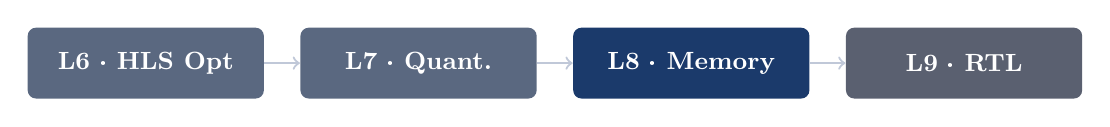
\begin{tikzpicture}[
  lbox/.style={rounded corners=3pt, minimum width=3.0cm, minimum height=0.9cm,
               align=center, font=\small\bfseries, text=white},
  node distance=0.45cm
]
  \node[lbox, fill=BoxGray]             (l6) {L6 \textperiodcentered\ HLS Opt};
  \node[lbox, fill=BoxGray,  right=of l6] (l7) {L7 \textperiodcentered\ Quant.};
  \node[lbox, fill=Navy,     right=of l7] (l8) {L8 \textperiodcentered\ Memory};
  \node[lbox, fill=MidGray,  right=of l8] (l9) {L9 \textperiodcentered\ RTL};
  \draw[->, thick, color=LtGray] (l6.east) -- (l7.west);
  \draw[->, thick, color=LtGray] (l7.east) -- (l8.west);
  \draw[->, thick, color=LtGray] (l8.east) -- (l9.west);
\end{tikzpicture}
\vspace{0.11cm}
{\color{Navy}\bfseries L8 --- Memory Hierarchy \& Cache}
\vspace{5pt}
\begin{itemize}\setlength{\itemsep}{2pt}
  \item[\color{Navy}$\blacktriangleright$]
    \textbf{OCM vs DDR:} on-chip memory (OCM, 256\,kB) is $\approx$100$\times$ faster
    than DDR --- knowing when your data fits in OCM matters
  \item[\color{Orange}$\blacktriangleright$]
    \textbf{L1/L2 cache behaviour:} how the Cortex-A9 caches interact
    with your bare-metal loops; cache-friendly access patterns
  \item[\color{Teal}$\blacktriangleright$]
    \textbf{Cache coherency with PL:}
    why \texttt{Xil\_DCacheFlushRange} and \texttt{Xil\_DCacheInvalidateRange}
    are mandatory around every DMA transfer
\end{itemize}
\vspace{0.07cm}
{\color{MidGray}\small\itshape
  Lab note: for your projects, try replacing \texttt{float} with
  \texttt{ap\_fixed} in your HLS kernel and measure the area and
  throughput improvement.}
\end{frame}

%% SLIDE 32
{
\setbeamercolor{background canvas}{bg=NavyDk}
\setbeamertemplate{footline}{%
  \vspace{2pt}%
  \hspace{0.6cm}{\color{LtGray}\fontsize{7.5}{9}\selectfont
    Hardware / Software Codesign \enspace|\enspace 2025/26 \enspace|\enspace IST}%
  \hfill%
  {\color{LtGray}\fontsize{7.5}{9}\selectfont\insertframenumber}%
  \hspace{0.5cm}\vspace{1pt}%
}
\begin{frame}[plain]
  \vspace{0.4cm}
  \begin{center}
    {\color{white}\fontsize{36}{42}\selectfont\textbf{Questions?}}
    \vspace{0.26cm}

    
\begin{tikzpicture}[
      rbox/.style={rounded corners=3pt, minimum width=2.6cm, minimum height=0.9cm,
                   align=center, font=\small\bfseries},
      node distance=0.3cm
    ]
      \node[rbox, fill=BoxGray, text=white] (a) {Range\\$\to$ $I$ bits};
      \node[rbox, fill=Orange,  text=white, right=of a] (b) {Target\\SNR};
      \node[rbox, fill=Teal,    text=white, right=of b] (c) {Sweep\\$W$};
      \node[rbox, fill=GreenHi, text=white, right=of c] (d) {Check\\resources};
    \end{tikzpicture}
  \end{center}
\end{frame}
}

\end{document}
